\chapter{Experiment with Getafix and jMoped}
	\label{CH_04}

We want to use model-checking tools to see if we can reduce the time requirement of Algorithm \ref{alg:doubleLoop}. Specifically, we choose the reachability property and append Algorithm \ref{alg:reachLine} to the end of Algorithm \ref{alg:doubleLoop}. The statement within the if statement has a label. Although the exact statement following that label is irrelevant, reaching this line means $OCounter$ satisfies the constrains in the condition block.

We experiment on several model-checking tools, including Interproc from \cite{_interproc_2011}, Berkeley Lazy Abstraction Software Verification Tool (Blast) from \cite{_mtc_2008}, Getafix from \cite{getafix} and jMoped from \cite{moped}. We can not get correct reachability results from Interproc and Blast, so we shift our focus onto Getafix and jMoped.

\renewcommand{\algorithmiccomment}[1]{// #1}
\begin{algorithm}
\begin{algorithmic}

\IF{value of $OCounter$ meets certain constrains}
\STATE reach: $OCounter$
\COMMENT{a label followed by a statement}
\ENDIF

\end{algorithmic}

\caption[Single loop]{Determine if $OCounter$ meets certain constrains.}
\label{alg:reachLine}
\end{algorithm}

\section{Getafix}
Getafix is a symbolic model checker for Boolean programs. Getafix only supports reachability check. It translates sequential and concurrent Boolean programs into Boolean formulae and uses the model-checker Mucke to solve the reachability problem symbolically using Boolean Decision Diagrams. 

\begin{figure}
\centering
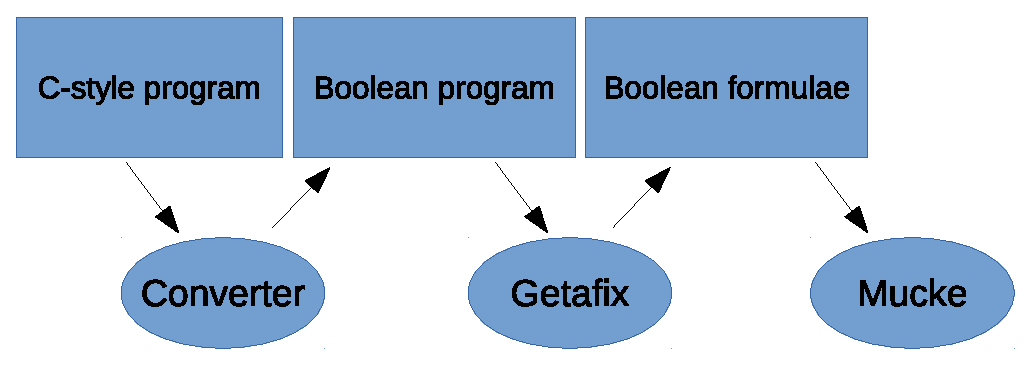
\includegraphics[scale=0.8]{Figures/workFlow}
\caption{Workflow of calculating information leakage with Getafix.}
\label{fig:workFlow}
\end{figure}

\subsection{The converter}
Input for Getafix are boolean programs, meaning it only supports binary variables which can be either 0 or 1. We represent our problem in C-style code, thus we need to translate it into boolean form. We implemented a converter to automate this process, and Figure \ref{fig:workFlow} shows the workflow we used to calculate information leakage using Getafix. The converter has three components, a parser, a built-in function generator and a piece of script which calls the first two components and assembles the output file. The converter has these properties:

\begin{enumerate}
\item The input to the converter is a C-style code file and a positive integer which represents the bit length. The converter supports 32 bits and less. Also note that the converter represents a number with bit length of $bitLength$ using $bitLength + 1$ bits. We do this so that we do not need to deal with the upper bound explicitly when writing a loop iterating from $0$ to $1<<bitLength - 1$.
\item The output of the converter is a boolean program which follows the syntax of Getafix input file.
\item In the language that we defined for the input file, we support only one variable type: non-negative decimal integer. Again we support the length up to 32 bits.
\item Our converter does not support function definitions. The input file has two parts, variable declarations block and statements block. The parser will print these blocks into the main function of the output boolean program. Also we require all variable declarations to appear before statements in the input code. Getafix input syntax has this requirement, and we decide to keep it in our converter.
\item We implement support for the following symbolic operators in the language: plus +, minus -, and \&, or $|$, xor \textasciicircum , greater than \textgreater, equal ==, less than \textless, not equal !=, greater than or equal \textgreater=, less than or equal \textless=, left shift \textless\textless and right shift \textgreater\textgreater.
\item We implement support for three control statements: if...else, while loop, goto and statements with labels. We currently do not support for loop, do...while loop, switch statements, break and continue, but these statements can be easily expressed using the supported ones.
\end{enumerate}

Input to the parser is a C-style code file and a desired bit length. Output of the parser is its corresponding boolean program which follows the syntax of Getafix input file. First we define the syntax of the input code and second we create the parser using flex and bison. The parser scans the input code and builds a syntax tree. Then the parser prints the syntax tree as a boolean program. The parser has three points worth noting:

\begin{table}
\begin{tabular}{|l|l|}
\hline
Input& Output  \\ \hline
var SMax = 16;     & \begin{tabular}[c]{@{}l@{}}decl SMax4,SMax3,SMax2,SMax1,SMax0;\\ Smax4, SMax3, SMax2, SMax1, SMax1 := 1,0,0,0,0;\end{tabular} \\ \hline
STemp = STemp - 5; & \begin{tabular}[c]{@{}l@{}}STemp4,STemp3,STemp2,STemp1,STemp0 := \\ minus(STemp4,STemp3,STemp2,STemp1,STemp0,0,0,1,0,1); \end{tabular} \\ \hline
\end{tabular}
\caption{Examples of input and output of the parser, with bit length of 4}
\label{tbl:parser-example}
\end{table}

\begin{enumerate}
\item When printing the output code, the parser ``stretches'' each variable and literal into its binary form. Assume the desired bit length is $bitLength$. We split each variable into $bitLength$ variables by copying the name of the variable $bitLength$ times and appending a counter value to each one. Also we convert a literal to its corresponding binary value and prepend it with zeros to reach the desired length. Table \ref{tbl:parser-example} contains an example of how the parser deals with a variable declaration.
\item In a boolean program, all operators operate on bit level, so we need to implement higher-level operators like plus, minus, greater than and left shift using operators that Getafix supports. In the parser, we print these high-level operators as function calls in the output boolean program, and the built-in function generator generates the body of the function. Table \ref{tbl:parser-example} also contains an example of how the parser deals with a high-level operator.
\item In the boolean code syntax which Getafix defines, function call plus the semicolon is defined as a statement, and another rule allows the code to assign a function call to an identifier, but function call itself is not an expression. This means that a function call can not work as an expression as in many other languages, and it leads to two problems: First, the decider expressions in if...else and while statements can not contain function calls. Second, parameters of a function call or operands to an operator can not be a function call. We automated a solution in the parser to the first problem, which assigns the decider expression to a temporary variable and use that variable as the decider, so we can use the C-style if...else and while in the input code. For the second problem, a possible solution would be to manage a set of internal temporary variables and assign each function call to a variable, but we did not implement it.
\end{enumerate}

Input to the built-in function generator is a desired bit length. Output is a set of high-level operators like plus and left shift implemented as functions. We do not track the necessary functions in the parser, as experiments with Getafix indicate that the uncalled functions affect little on the execution time. Listing \ref{lst:isGT} shows a sample function by the generator.

\lstset{language=C}  
\begin{lstlisting}[float=h, caption={Greater than operator as a function in boolean program with bit length of 2.},label=lst:isGT]
bool isGT(left2,left1,left0,right2,right1,right0)
begin
if (left2 != right2) then
	if (left2 = 1) then return 1; fi
else 
	if (left1 != right1) then
		if (left1 = 1) then	return 1; fi
	else 
		if (left0 != right0) then
			if (left0 = 1) then	return 1; fi
fi	fi	fi
return 0;
end
\end{lstlisting}

Input to the third component, a piece of script, is a C-style code file and a desired bit length. Output of the script is a boolean program ready for Getafix to process. The script first passes the bit length to the built-in function generator and redirects its output to the output file. Then the script passes both the input to the parser and appends its output to the output file. At this point the output is complete.

\section {jMoped}
jMoped is a model checker which checks for coverage in Java programs. The authors implemented it as a plug-in for eclipse, using its UI for parameters and output display. We rewrite our tests in Java so that we can use jMoped on them.

\section{Tests and results}
Before we have the converter, we coded a few test cases manually and Getafix gave us the correct answers. Now with the converter we can run more complicated tests and see if Getafix is a good solution to the problem of calculating information leakage. As with jMoped, we rewrite the tests in Java. We decide to run the eight test cases from paper \cite{Plas11}. In each test, $O$ represents the output of the test program, and $S$ is the input. Also in the tables, opt refers to the final optimization in the previous chapter, and we set the maximum execution time to 600 seconds. 

We did our tests on a laptop computer, and key hardware specifications are:
\begin{description}
  \item[Model] Lenovo ideapad Y580-IFI
  \item[CPU] Intel Core i5-3210M @ 2.5GHz
  \item[Memory] 4GBytes DDR3-1600 $\times$ 2
\end{description}

And the software specifications are:
\begin{description}
  \item[OS] Ubuntu 14.04 LTS 32-bit
  \item[Getafix] Version information not available. Source code retrieved on 2014/4/10
  \item[Mucke] Version 0.4.4
  \item[Eclipse] Eclipse juno sr2
  \item[jMoped] Version 2.0.2
\end{description}

For Getafix, we time the entire process from converter to Mucke using the time command in bash and record the elapsed wall time. For jMoped, we record the elapsed wall time which jMoped reports.

\subsection{Sanity check}
Listing \ref{lst:sanity} shows the code we use. In this test, $O$ remains constant unless $S$ is within a certain range. The program has 16 different outputs, ranging from $4$ to $19$. We can use the optimization in this test, and the timing results are in Table \ref{tbl:sanity}.

\lstset{language=C}  
\begin{lstlisting}[float=!h, caption={Sanity check test program.},label=lst:sanity]
var base = 4;
if(S < 16){O = base+ S;}
else{O = base;}
\end{lstlisting}

\begin{table}[!h]
\begin{center}
\begin{tabular}{|l|l|l|l|l|}
\hline
bit length(bit) & Getafix(s) & Getafix opt(s) & jMoped(s) & jMoped opt(s) \\ \hline
6 & 41.264 & 2.093 & 9.32 & 0.42 \\ \hline
7 & 235.640 & 3.378 & 62.07 & 0.53 \\ \hline
8 & \textgreater600 & 6.448 & 326.12 & 0.88 \\ \hline
9 &  & 13.491 & JVM terminates & 1.69 \\ \hline
10 &  & 27.479 &  & 3.05 \\ \hline
11 &  & 61.871 &  & 6.23 \\ \hline
12 &  & 140.115 &  & 14.80 \\ \hline
13 &  & 302.96 &  & 35.17 \\ \hline
14 &  & 580.982 &  & 78.29 \\ \hline
15 &  & \textgreater600 &  & 181.82 \\ \hline
16 &  &  &  & 444.17 \\ \hline
17 &  &  &  & JRE Error \\ \hline
\end{tabular}
\end{center}
\caption{Timing results for sanity check.}
\label{tbl:sanity}
\end{table}

\subsection{Implicit flow}
Listing \ref{lst:implicit} shows the code. This test copies the value of $S$ to $O$ indirectly through the if statement when $S$ is less than $7$. For other $S$ values, $O$ is $0$. The program has 7 different outputs, ranging from $0$ to $6$. We can use the optimization in this test, and the timing results are in Table \ref{tbl:implicit}.

\lstset{language=C}  
\begin{lstlisting}[float=!h, caption={Implict flow test program.},label=lst:implicit]
O = 0;
if(S == 0){O = 0;}
else{if(S == 1){O = 1;}
	else{if(S == 2){O = 2;}
		else{if(S == 3){O = 3;}
			else{if(S == 4){O = 4;}
				else{if(S == 5){O = 5;}
				  else{if(S == 6){O = 6;}
}	}	}	} 	} }
\end{lstlisting}

\begin{table}[!h]
\begin{center}
\begin{tabular}{|l|l|l|l|l|}
\hline
bit length(bit) & Getafix(s) & Getafix opt(s) & jMoped(s) & jMoped opt(s) \\ \hline
6 & 58.834 & 2.937 & 11.87 & 0.47 \\ \hline
7 & 289.919 & 8.265 & 63.56 & 0.58 \\ \hline
8 & \textgreater600 & 22.644 & 325.76 & 0.97 \\ \hline
9 &  & 61.464 & \textgreater600 & 1.86 \\ \hline
10 &  & 182.130 &  & 3.57 \\ \hline
11 &  & 429.298 &  & 7.21 \\ \hline
12 &  & \textgreater600 &  & 15.75 \\ \hline
13 &  &  &  & 36.31 \\ \hline
14 &  &  &  & 81.53 \\ \hline
15 &  &  &  & 182.01 \\ \hline
16 &  &  &  & 415.69 \\ \hline
17 &  &  &  & \textgreater600 \\ \hline
\end{tabular}
\end{center}
\caption{Timing results for implicit flow.}
\label{tbl:implicit}
\end{table}

\subsection{Mix and duplicate}
Listing \ref{lst:mix} shows the code. This test first calculates the XOR value of the two halves of $S$ (mix) and second duplicates this XOR value twice in $O$ (duplicate). The output count depends on the bit length, and at $8$ bits, it has $2^{4} = 16$ different outputs. We can use the optimization in this test, and the timing results are in Table \ref{tbl:mix}.

\lstset{language=C}  
\begin{lstlisting}[float=!h, caption={Mix and duplicate test program at 8 bits.},label=lst:mix]
O = ((S >> 4) ^ S) & 15;
O = O | O << 4;
\end{lstlisting}
\begin{table}[htbp]
\begin{center}
\begin{tabular}{|l|l|l|l|l|}
\hline
bit length & Getafix(s) & Getafix opt(s) & jMoped(s) & jMoped opt(s) \\ \hline
4 & 2.719 & 0.983 & 1.14 & 0.38 \\ \hline
6 & 44.728 & 3.719 & 32.94 & 0.63 \\ \hline
8 & \textgreater600 & 32.931 & JVM terminates & 1.97 \\ \hline
10 &  & Memory alloc error &  & 9.77 \\ \hline
12 &  &  &  & 69.01 \\ \hline
14 &  &  &  & JVM terminates \\ \hline
\end{tabular}
\end{center}
\caption{Timing results for mix and duplicate.}
\label{tbl:mix}
\end{table}

\subsection{Masked copy}
Listing \ref{lst:masked} shows the code. In this test, $O$ is $S$ with its lower half set to $0$, or ``masked'' out. The output count depends on the bit length, and at $8$ bits, it has $2^{4} = 16$ different outputs. We can use the optimization in this test, and the timing results are in Table \ref{tbl:masked}.

\lstset{language=C}  
\begin{lstlisting}[float=!h, caption={Masked copy test program at 8 bits.},label=lst:masked]
O = S & 240;
\end{lstlisting}

\begin{table}[!h]
\begin{center}
\begin{tabular}{|l|l|l|l|l|}
\hline
bit length & Getafix(s) & Getafix opt(s) & jMoped(s) & jMoped opt(s) \\ \hline
4 & 1.728 & 0.752 & 0.61 & 0.23 \\ \hline
6 & 38.244 & 1.386 & 10.29 & 0.35 \\ \hline
8 & \textgreater600 & 5.254 & 320.87 & 0.81 \\ \hline
10 &  & 39.136 & JVM terminates & 2.45 \\ \hline
12 &  & 247.135 &  & 11.78 \\ \hline
14 &  & \textgreater600 &  & 57.08 \\ \hline
16 &  &  &  & 327.95 \\ \hline
18 &  &  &  & JRE fatal error \\ \hline
\end{tabular}
\end{center}
\caption{Timing results for masked copy.}
\label{tbl:masked}
\end{table}

\subsection{Binary search}
Listing \ref{lst:bin} shows the code. This test leaks the upper half of $S$ to $O$ through binary search. The output count depends on the bit length, and at $8$ bits, it has $2^{4} = 16$ different outputs. We can use the optimization in this test, and the timing results are in Table \ref{tbl:bin}.

\lstset{language=C} 
\begin{lstlisting}[float=!h, caption={Binary search test program at 8 bits.},label=lst:bin]
if(O + 128 <= S){O = O + 128;}
if(O + 64 <= S){O = O + 64;}
if(O + 32 <= S){O = O + 32;}
if(O + 16 <= S){O = O + 16;}
\end{lstlisting}

\begin{table}[!h]
\begin{center}
\begin{tabular}{|l|l|l|l|l|}
\hline
bit length & Getafix(s) & Getafix opt(s) & jMoped(s) & jMoped opt(s) \\ \hline
4 & 3.359 & 1.094 & 0.91 & 0.33 \\ \hline
6 & 136.074 & 5.947 & 28.26 & 0.64 \\ \hline
8 & \textgreater600 & 65.235 & JVM terminates & 2.32 \\ \hline
10 &  & \textgreater600 &  & 13.53 \\ \hline
12 &  &  &  & 99.49 \\ \hline
14 &  &  &  & JVM terminates \\ \hline
\end{tabular}
\end{center}
\caption{Timing results for binary search.}
\label{tbl:bin}
\end{table}

\subsection{Electronic purse}
Listing \ref{lst:electronic} shows the code. Assume $S$ is the account balance, we set the deduction to $5$, and output $O$ represents the number of times one can debit such an amount.  In this test we set $SMax$ to $19$,and the program has $4$ outputs, ranging from $0$ to $3$. We can use the optimization in this test, and the timing results are in Table \ref{tbl:electronic}.

\lstset{language=C}  
\begin{lstlisting}[float=!h, caption={Electronic purse test program.},label=lst:electronic]
O = 0;
while(S >= 5){
	S = S - 5;
	O = O + 1;
}
\end{lstlisting}

\begin{table}[!h]
\centering
\begin{tabular}{|l|l|l|l|l|}
\hline
{bit length(bit)} & Getafix(s) & {Getafix opt(s)} & jMoped(s) & {jMoped opt(s)} \\ \hline
{5} & {10.411} & {2.781} & {1.70} & {0.31} \\ \hline
\end{tabular}
\caption{Timing results for electronic purse.}
\label{tbl:electronic}
\end{table}

\subsection{Sum query}
Listing \ref{lst:sum} shows the code. This test leaks the sum of its three inputs to $O$. We set $S1, S2$ and $S3$ to be less than $10$, so the program has $28$ outputs ranging from $0$ to $27$. We can use the optimization in this test, and the timing results are in Table \ref{tbl:sum}.

\lstset{language=C}  
\begin{lstlisting}[float=!h, caption={Sum query test program.},label=lst:sum]
O = S1 + S2 + S3;
\end{lstlisting}

\begin{table}[!h]
\centering
\begin{tabular}{|l|l|l|l|l|}
\hline
{bit length(bit)} & Getafix(s) & {Getafix opt(s)} & jMoped(s) & {jMoped opt(s)} \\ \hline
5 & 225.400 & 33.488 & 21.12 & 2.60	\\ \hline
\end{tabular}
\caption{Timing results for sum query.}
\label{tbl:sum}
\end{table}

\section{Results summary}
From the seven test programs and timing results, we can conclude the following points:
\begin{enumerate}
\item At the same bit length, jMoped is faster than Getafix. 
\item The optimization can reduce execution time for jMoped and Getafix greatly.
\item The best result we get is using jMoped with the optimization, but still the time growth is exponential.
\end{enumerate}

